\section{Requirements analysis} \label{sec:requirements}

% Simplicity
% Low cost
% Robust (SW & HW)
% Modularity
% Visually/Physically based
% Control:
% - DCS
% - Local & Remote control
% - Velocity & Position

When considering the development of any practical demonstrator, some general requirements should be taken into consideration due to the scope of such products.
These become even more relevant when the demonstrator is designed for educational purposes, as this is one such scenario.

The following subsections will delve into the main requirements of the project, explaining why they are being considered a requirement, how they were dealt with during development phase, what difficulties were encountered to meet such need and in which manner each requirement influenced the final system.

\subsection{Simplicity}

The most important characteristic every demonstrator should own is simplicity.
No matter how complex or extensive the concept might be, good demonstrators are conceptually simple.
Designs that focus solely on the concept at hand and leave out superfluous functionality tend to be more effective at conveying the main message.
Having the ability to further explore the concept beyond the initial scope of the demonstrator by extending its capabilities could be an advantage, but only when the implications of doing so do not hurt the initial simplicity.

To contemplate different approaches based on simple concepts is crucial to ensure the end result is focused on the correct concept.
It is also very important to not allow underlying characteristics or design choices to outweigh the core concept.

\subsection{Low-cost} \label{sec:low-cost}

Demonstrators whose purpose is to serve as a first contact mechanism under an educational directive should be as low-cost as possible.
Accidents, bad practices or the simple lack of necessary knowledge can lead students and first-timers to, unintentionally, damage educational equipment.

Students tend to learn more easily when left to their own experiments, learning by themselves how things work and how to operate them. % TODO Cite something
For this to be possible, educational equipment should not impose limitations on the user freedom and, to meet such goal, low-cost is generically the best option.
Students must be able to experiment and learn without having to constantly worry about possible damage to expensive equipment.

Also, when looking through the point of view of the education institution, the best way to provide students with such contact is to allow them to individually, or in small groups, utilise the equipment.
Ideally, one equipment per work desk would be used, which quickly increases the amount of demonstrators the institution should own and, consequently, the expenses on acquiring them.
As such, keeping a low-cost vision for these equipment will help education institutions to provide their students wit the best experience possible.

\subsection{Modularity}

Designing a system based on well defined modules is always a good thing.
Modularity helps divide the most complex systems into several parts, which are easier to handle and understand.
This characteristic also helps reduce costs, especially when considering the integration of pre-made modules, instead of developing new ones.

When there is possibility to design a product that reuses components and modules available on the market, production, maintenance and repairs become simpler and cost-effective.
With this approach, a damaged physical module can simply be replaced and software modules become easier to work with.
When developing software modules, one needs to pay close attention to the planned boundaries of each module, making sure their functionality is entirely self-contained.
This way, if we wish to replace a physical module we can also simply swap the respective software module with a new one, targeted at the new physical module.

\subsection{DCS based architecture}

With our aim being the influence of network cycle time on control applications, it's imperative for us to use an architecture that resembles a Distributed Control System (DCS).
An example of a DCS architecture can be seen in \autoref{fig:dcs-architecture} (page \pageref{fig:dcs-architecture}).
It only makes sense to evaluate such influence on systems where it is applicable, meaning, we must replicate a real world case where the usage of an RTE network might actually influence the system performance.
With this in mind, we decided to replicate the concept of a networked servo drive controlled from a centralised processing unit, with the ability to close the control loop either locally on the servo drive (the current typical scenario) or remotely on the processing unit.

\begin{figure}[htp]
	\centering
	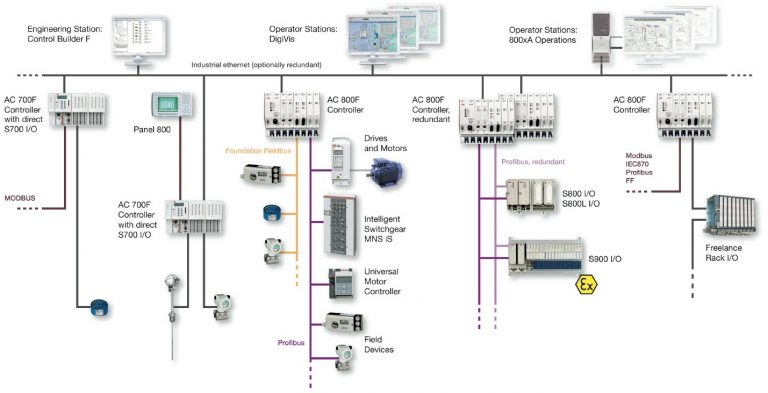
\includegraphics[width=0.8\textwidth]{Architecture-of-DCS.jpg}
	\caption{Example of a DCS architecture (adapted from \cite{misc:dcs-architecture})}
	\label{fig:dcs-architecture}
\end{figure}

\subsubsection{Local Vs. Remote control} \label{subsec:local_remote}

In order to better visualise the effects of network cycle time in control applications, a baseline should be defined to serve as a basis for comparison.
The field device will be capable of performing full control of position and/or velocity of the motor or serve as a simple remotely controlled servo drive.

With the first configuration (local control), the field device will receive only the set-point values from the RTE and then perform the position/velocity control of the motor using an internal control algorithm.
This will generate a baseline dataset of control performance, which is expected to barely be affected by the network cycle time.

The second configuration (remote control) will use the field device as a simple servo drive, without using its internal control algorithm.
It shall receive the velocity reference to be applied to the motor from the RTE network and send back the decoded position/velocity, acquired from the motor's incremental encoder, through the same network, as a feedback variable.
This will mean the control loop will be closed on the remote processing unit, making this loop's output and feedback values traverse the RTE network.
It's expected for this configuration to be mildly affected by the network cycle time, even though we will probably need to use unusually large values of this parameter to obtain relevant changes in the control performance.

\subsubsection{Velocity and position control}

In order to give the demonstrator a bit more flexibility and broaden the range of conceptual experiments, we aim to develop a demonstrator capable of controlling the motor's velocity and position.
To clarify, we do not plan to provide simultaneous control of both these movement types.
Having the ability to chose the type of movement we want to control each time the field device is powered on will allow us to develop new and interesting experiments, including more advanced movement control.
